\documentclass{standalone}
\usepackage{tikz}
\usepackage{pgfplots}
\pgfplotsset{compat=1.16}

\begin{document}
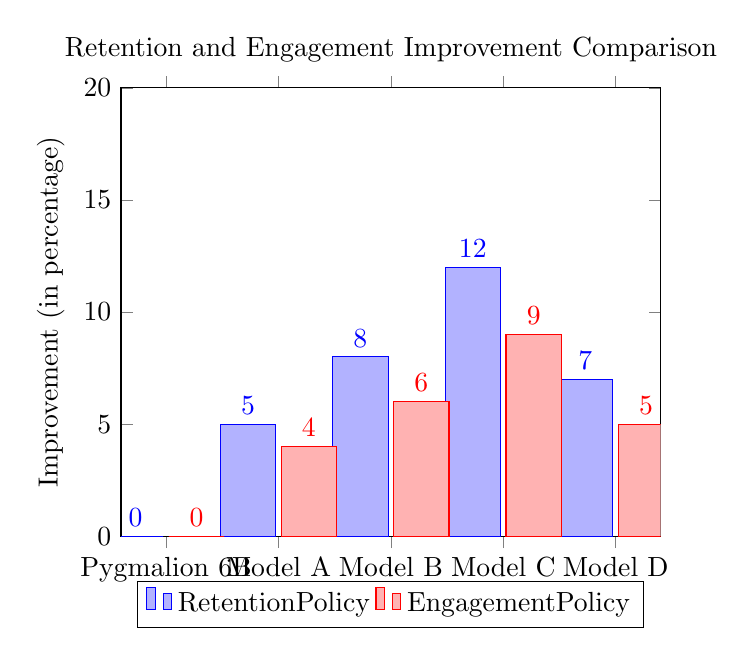
\begin{tikzpicture}
    \begin{axis}[
        ybar,
        symbolic x coords={Pygmalion 6B, Model A, Model B, Model C, Model D},
        xtick=data,
        nodes near coords,
        nodes near coords align={vertical},
        ylabel={Improvement (in percentage)},
        title={Retention and Engagement Improvement Comparison},
        ymin=0,
        ymax=20,
        bar width=20pt,
        legend style={at={(0.5,-0.1)}, anchor=north,legend columns=-1},
    ]
        \addplot coordinates {(Pygmalion 6B, 0) (Model A, 5) (Model B, 8) (Model C, 12) (Model D, 7)};
        \addlegendentry{RetentionPolicy}
        
        \addplot coordinates {(Pygmalion 6B, 0) (Model A, 4) (Model B, 6) (Model C, 9) (Model D, 5)};
        \addlegendentry{EngagementPolicy}
    \end{axis}
\end{tikzpicture}
\end{document}